\documentclass[11pt]{exam}
\usepackage[utf8]{inputenc}
\usepackage[a4paper,top=2cm,left=2cm,right=2cm,bottom=2cm]{geometry}
\usepackage{import}
\usepackage[T1]{fontenc}
\usepackage[german,ngerman]{babel}
\usepackage[table]{xcolor}
\usepackage{amsthm, esvect}
\usepackage{mathtools}
\RequirePackage{amssymb, amsfonts, amsmath, latexsym, verbatim, xspace}
\usepackage{systeme}
\usepackage{multicol}
\usepackage{multirow}
\usepackage{framed}
\usepackage{array}
\usepackage{ragged2e}
\usepackage{graphicx}
\usepackage{pdflscape}
\usepackage{epstopdf}
\usepackage{booktabs}
\usepackage{pdfpages}
\usepackage{float} % Allows putting an [H] in \begin{figure} to specify the exact location of the figure
\usepackage{wrapfig} % Allows in-line images such as the example fish picture
\usepackage{tikz, graphicx} % tikz
\usepackage[position=top]{subfig}
\usepackage[bookmarks=true]{hyperref}%Links
\usepackage{enumerate}
\usepackage{enumitem}
\usepackage[german,ruled,vlined,linesnumbered,algosection]{algorithm2e}
\usepackage[labelfont=sf]{caption}
\usepackage{lmodern}
\usepackage{lscape}
\usepackage{tabularx}
\usepackage{systeme}
\usepackage{hhline}
\usepackage{subfiles}
\usepackage{stackengine}
\usepackage{setspace}
\usepackage{MnSymbol}
\usepackage{tcolorbox}
\usepackage{bbm}
\usepackage{url}
\usepackage{xparse}
\usepackage{sectsty}
\usepackage{array}
\usepackage{ragged2e}
\usepackage{listings} %Stellt Code-Snippets sauber dar

% definiert die Sprache
\selectlanguage{German}

% add command for different dates in Swiss fashion
\newcommand{\monthwordlong}[1]{\ifcase#1 \or Januar\or Februar\or März\or April\or Mai\or Juni\or Juli\or August\or September\or Oktober\or November\or Dezember\fi}
\newcommand{\monthwordshort}[1]{\ifcase#1\or Jan\or Feb\or Mar\or Apr\or Mai\or Jun\or Jul\or Aug\or Sept\or Okt\or Nov\or Dez\fi}
\newcommand{\datelong}{\number\day.\:\monthwordlong{\the\month}\:\number\year}
\newcommand{\dateshort}{\number\day.\:\monthwordshort{\the\month}\:\number\year}

% define color of links inside a text
\definecolor{linkblue}{RGB}{0, 0, 80}
\definecolor{plotblue}{RGB}{100, 100, 255}
\definecolor{myblue}{RGB}{8,164,214}
\definecolor{myred}{RGB}{143,42,41}
\definecolor{forestgreen}{RGB}{34,139,34}
\definecolor{highdive}{RGB}{10,169,194}
\definecolor{charcoal}{RGB}{74,74,74}
\hypersetup{
	colorlinks=true,
	linkcolor=linkblue,
	filecolor=magenta,
	urlcolor=plotblue,
	citecolor=linkblue,
	pdfpagemode=FullScreen,
}


\lstdefinestyle{mystyle}{ % definiert den style des Code-Snippets
	%backgroundcolor=\color{backcolour},
	%commentstyle=\color{codegreen},
	%keywordstyle=\color{magenta},
	%numberstyle=\tiny\color{codegray},
	%stringstyle=\color{codepurple},
	basicstyle=\ttfamily\footnotesize,
	breakatwhitespace=false,
	breaklines=true,
	captionpos=b,
	keepspaces=true,
	%numbers=left,
	%numbersep=5pt,
	showspaces=false,
	showstringspaces=false,
	showtabs=false,
	tabsize=4
}
\lstset{style=mystyle}
\qformat{\Large\textbf{Aufgabe \thequestion\hfill\thepoints}}
\newlist{partes}{enumerate}{3}
\setlist[partes]{label=(\alph*)}
\newcommand{\parte}{\item}
\newlist{subpartes}{enumerate}{3}
\setlist[subpartes]{label=\roman*)}
\newcommand{\subparte}{\item}
\setlist[enumerate,1]{%(
	leftmargin=*, itemsep=12pt, label={\textbf{\arabic*.)}}}
\newcommand\answerbox{%%
	\fbox{\rule{2in}{0pt}\rule[-0.1ex]{0pt}{4ex}}}
\pointpoints{Punkt}{Punkte}
\hqword{Frage:}
\hpword{Mögliche Punkte:}
\hsword{Erreicht:}
\htword{Total}
\renewcommand*\half{.5}
\renewcommand{\solutiontitle}{\noindent\textbf{Lösung:}\par\noindent}

% Graphed boxes
\newcommand{\karos}[2]{
  \begin{tikzpicture}
    \draw[step=0.4cm,color=cyan,dotted] (0,0) grid (#1 cm ,#2 cm);
  %  \draw((#1)/2 cm,0)--((#1)/2 cm,/#2)/2cm)
  \end{tikzpicture}
}
\usetikzlibrary{arrows, petri, topaths, graphs}
\linespread{1.2} % Line spacing

%=========================================================
\newenvironment{parcols}[1][]{
    \begin{parts}\begin{multicols}{#1}
}{
    \end{multicols}\end{parts}
}
%=========================================================
\newenvironment{itemcols}[1][]{
	\begin{itemize}\begin{multicols}{#1}
		}{
	\end{multicols}\end{itemize}
}

%=========================================================
\newcommand{\antwort}[1]{
	{\setlength{\textwidth}{\textwidth}\fillwithgrid{#1cm}\vspace{5pt}}
}

%=========================================================
% Karriertes Papier für Antwort MIT OVERLAY
\tcbuselibrary{breakable,skins}
\usetikzlibrary{mindmap,trees}
\newlength\tindent
\setlength{\tindent}{\parindent}
\setlength{\parindent}{0pt}
\setlength{\parskip}{0pt}

\newtcolorbox{gridspace}[1]{%
	enhanced,
	breakable,
	blanker,
	boxrule=0pt,
	left=5mm,
	right=5mm,
	top=5.75mm,
	bottom=0mm,
	boxsep=0pt,
	height=#1cm,
	width=16cm,
	before upper={
		\begingroup
		\setlength{\baselineskip}{5.75mm}
		\setlength{\parskip}{0pt}
		\setlength{\lineskip}{0pt}
		% keep every paragraph on the grid rhythm
		%\everypar{\vspace{0pt}\strut}
		% math formulas shifted by one grid row
		\let\oldbracketopen\[
		\renewcommand{\[}{\vspace{-5mm}\oldbracketopen}
		% Align displayed formulas to the grid
		\setlength{\abovedisplayskip}{0pt}
		\setlength{\belowdisplayskip}{0pt}
		\setlength{\abovedisplayshortskip}{0pt}
		\setlength{\belowdisplayshortskip}{0pt}
		% Enumerate follows the same rhythm
		\setlist[enumerate]{leftmargin=6mm,itemsep=0mm,topsep=0pt,parsep=0pt,partopsep=0pt}
		\setlist[itemize]{leftmargin=6mm,itemsep=10mm,topsep=0pt,parsep=0pt,partopsep=0pt}},
	after upper={
		\endgroup},
	underlay={
		\draw[step=5mm,color=gray!55] (interior.south west) grid (interior.north east);}
}

\pagestyle{headandfoot}
\firstpageheader{}{}{\teacher}
\runningheader{}{}{\teacher}
\firstpagefooter{}{}{Seite \thepage\:von \numpages}
\runningfooter{}{}{Seite \thepage\:von \numpages}
%%
% Math Arrows
%%
\newcommand{\same}{\ensuremath{\Longleftrightarrow}}
\renewcommand{\to}{\ensuremath{\longrightarrow}}
\newcommand{\qsame}{\quad\same\quad}
\newcommand{\dsame}{\ensuremath{:\Leftrightarrow}}
\newcommand{\qdsame}{\quad\dsame\quad}
\newcommand{\ldsame}{\ensuremath{:\Longleftrightarrow}}
\newcommand{\samedef}{\ensuremath{\us {\text{def}} \Leftrightarrow}}
\newcommand{\qsamedef}{\quad\samedef\quad}
\newcommand{\lsamedef}{\ensuremath{\us {\text{def}} \Longleftrightarrow}}
\newcommand{\qlsamedef}{\quad\lsamedef\quad}


%%
% Mengendefinitionen
%%
\newcommand{\M}{\ensuremath{\mathcal{M}}}
\newcommand{\N}{\ensuremath{\mathbb{N}}}
\newcommand{\Z}{\ensuremath{\mathbb{Z}}}
\newcommand{\Q}{\ensuremath{\mathbb{Q}}}
\newcommand{\I}{\ensuremath{\mathbb{I}}}
\newcommand{\R}{\ensuremath{\mathbb{R}}}
\newcommand{\C}{\ensuremath{\mathbb{C}}}
\renewcommand{\S}{\ensuremath{\mathbb{S}}}
\newcommand{\Prim}{\ensuremath{\mathbb{P}}}
\newcommand{\0}{\ensuremath{\emptyset}}
\renewcommand{\Re}{\ensuremath{\operatorname{Re}}}
\renewcommand{\Im}{\ensuremath{\operatorname{Im}}}
\newcommand{\strich}{\ensuremath{\big\vert}}

%%
% Mengenoperation
%%
\renewcommand{\nin}{\not\in}


%%
% Logisches Und und Oder
%%
\newcommand{\sand}{\ensuremath{\; \land \;}}
\newcommand{\sor}{\ensuremath{\; \lor \;}}
\renewcommand{\*}{\ensuremath{\cdot}}
\newcommand{\oder}{\vee}
\newcommand{\n}{\neg}
\newcommand{\und}{\wedge}


%%
% Bei Integral, Summe,... die Grenzen über bzw.
% unter das Zeichen
%%
\renewcommand{\d}[1]{\ensuremath{\operatorname{d}\!{#1}}}
\newcommand{\Sum}{\sum\limits}
\newcommand{\Prod}{\prod\limits}
\newcommand{\Min}{\min\limits}
\newcommand{\Max}{\max\limits}
\newcommand{\Lim}{\lim\limits}
\newcommand{\Inf}{\inf\limits}
\newcommand{\Sup}{\sup\limits}
\newcommand{\Liminf}{\liminf\limits}
\newcommand{\Limsup}{\limsup\limits}
%\renewcommand{\Cup}{\bigcup\limits}
%\renewcommand{\Cap}{\bigcap\limits}
\newcommand{\Otimes}{\bigotimes\limits}
\newcommand{\Oplus}{\bigoplus\limits}


%%
% Arcus Cotangens, Logarithmus
%%
\let\oldsin\sin
\renewcommand{\sin}[1]{\oldsin{\left(#1\right)}}
\let\oldcos\cos
\renewcommand{\cos}[1]{\oldcos{\left(#1\right)}}
\let\oldtan\tan
\renewcommand{\tan}[1]{\oldtan{\left(#1\right)}}
\let\oldarcsin\arcsin
\renewcommand{\arcsin}[1]{\oldarcsin{\left(#1\right)}}
\let\oldarccos\arccos
\renewcommand{\arccos}[1]{\oldarccos{\left(#1\right)}}
\let\oldarctan\arctan
\renewcommand{\arctan}[1]{\oldarctan{\left(#1\right)}}
\let\oldln\ln
\renewcommand{\ln}[1]{\oldln{\left(#1\right)}}
\newcommand{\Log}[2]{\ensuremath{\operatorname{log}_{#1}\left(#2\right)}}
\newcommand{\e}{\operatorname{e}}
\renewcommand{\exp}[1]{\ensuremath{\operatorname{\e}^{#1}}}


%%
% Griechische Buchstaben
%%
\renewcommand{\epsilon}{\ensuremath{\varepsilon}}
\renewcommand{\phi}{\varphi}
\renewcommand{\l}{\lambda}
\renewcommand{\t}{\tau}


%%
% Bezeichnungen
%%
\newcommand{\Rgn}{\R_{>0}} % R grösser Null
\newcommand{\Rad}{\operatorname{Rad}}   % Radikal
\newcommand{\kgV}{\operatorname{kgV}}   % Kleinster gemeinsame Vielfache
\newcommand{\ggT}{\operatorname{ggT}}   % Grösster gemeinsame Teiler
\newcommand{\winkel}{\sphericalangle}          % Winkelsymbol
\DeclarePairedDelimiter\abs{\lvert}{\rvert} % besserer Betrag
\makeatletter
\let\oldabs\abs
\def\abs{\@ifstar{\oldabs}{\oldabs*}}
\makeatother


%%
% Vektorgeometrie
%%
\renewcommand{\v}[1]{\vv{#1}}       % besserer Pfeil über Buchstaben
\renewcommand{\vec}[2]{\begingroup\renewcommand{\arraystretch}{1}\left(\begin{array}{c} #1 \\ #2 \end{array}\right)\endgroup}   % two dimensional vector
\renewcommand{\Vec}[3]{\begingroup\renewcommand{\arraystretch}{1}\left(\begin{array}{c} #1 \\ #2 \\ #3 \end{array}\right)\endgroup}      % three dimensional vector


%%
% Text
%%
\newcommand*{\Ueq}[1]{\mathrel{\mathop{=}\limits_{\text{#1}}}}
\newcommand*{\Oeq}[1]{\mathrel{\stackrel{\text{#1}}{=}}}
\newcommand{\utext}[2]{\underbrace{#1}_{\substack{#2}}}
\newcommand{\otext}[2]{$\overbrace{\textrm{#1}}^{\textrm{#2}}$}
\newcommand{\lineortext}[1]{\hspace{0,1cm}\underline{\hspace{0.1cm}\hphantom{#1}\hspace{0.1cm}}\hspace{0,1cm}} % Lückentext erstellen
\newcommand{\gap}[1]{\rule{#1 cm}{1pt}}
\graphicspath{{data-geometrie/}}
%=========================================================
\newcommand{\theme}{Trigonometrie}
\newcommand{\teacher}{Jonas Guler}
%=========================================================
\begin{document}
\fontsize{14}{14}\selectfont
\begin{center}
    \huge\bf\theme
\end{center}

\begin{questions}
%=========================================================
%-------------------TESTFRAGEN
%=========================================================
\question[5] %Rhyn S2 A9f
\begin{minipage}{0.6\linewidth}
	Berechne alle fehlenden Seiten und Winkel, wenn
	\[c=7.68\quad\text{ und }\quad\alpha=3\beta\]
	gegeben sind.
\end{minipage}
\hfill
\begin{minipage}{0.35\linewidth}
	\centering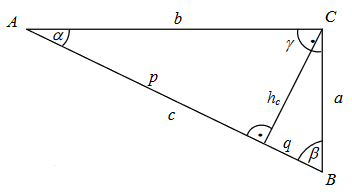
\includegraphics[scale=0.6]{trigo-dreieck.png}
\end{minipage}


%---------------------------------------------------------
\question[6] %Rhyn S2 A10f
\begin{minipage}{0.6\linewidth}
	Berechne alle fehlenden Seiten und Winkel, wenn
	\[h_c=9.1\quad\text{ und }\quad p=6\]
	gegeben sind.
\end{minipage}
\hfill
\begin{minipage}{0.35\linewidth}
	\centering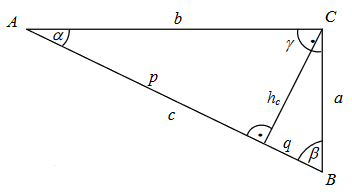
\includegraphics[scale=0.6]{trigo-dreieck.png}
\end{minipage}


%---------------------------------------------------------
\question[5] % Funktionsgraphen
\textbf{Beachte:} Lösungswege mit Hilfe des Taschenrechners geben keine Punkte!
\begin{parts}
	\part Zeichne den Winkel $\alpha=230^\circ$ im Einheitskreis ein und gib den Sinus-, Cosinus- und Tangenswert von $\alpha$ an.
\end{parts}
\vspace{5pt}
\begin{figure}[H]
	\begin{tikzpicture}[cross/.style={draw, cross out, minimum size=2*(#1-1pt), inner sep=0pt, outer sep=0pt}, x=10mm, y=10mm,
		>=latex,   %Voreinstellung für Pfeilspitzen
		font= \footnotesize, scale=3]
		%Raster zeichnen
		% \draw [color=gray!50]  [step=7.5mm] (-1.3,-5.3) grid (14.8,5.8);
		% Achsen zeichnen
		\draw[->,thick] (-1.1,0) -- (1.2,0) node[right, below] {\normalsize $x$};
		\draw[->,thick] (0,-1.1) -- (0,1.2) node[above, left] {\normalsize $y$};
		% Achsen beschriften
		\foreach \x in {-1,1} \draw (\x,-.1) -- (\x,.1) node[below=4pt] {$\x$};
		\foreach \y in {-1,1} \draw (-.1,\y) -- (.1,\y) node[left=4pt] {$\y$};
		% Besserer Ursprung
		\draw[color=black] (0pt,-7pt) node[right] {$0$};
		%Funktionen zeichnen:
		\clip(-1.1,-1.1) rectangle (1.1,1.1); %Bildbereich
		\draw circle [radius=1];
	\end{tikzpicture}
\end{figure}
\begin{parts}
	\setcounter{partno}{1}
	\part Berechne alle Winkel $\beta$ zwischen $0^\circ$ und $360^\circ$ für welche gilt: \[\cos{\beta}=-0.65\]
\end{parts}
\begin{figure}[H]
	\begin{tikzpicture}[cross/.style={draw, cross out, minimum size=2*(#1-1pt), inner sep=0pt, outer sep=0pt}, x=10mm, y=10mm,
		>=latex,   %Voreinstellung für Pfeilspitzen
		font= \footnotesize, scale=3]
		%Raster zeichnen
		\draw [color=gray!50]  [step=2mm] (-1,-1) grid (1,1);
		% Achsen zeichnen
		\draw[->,thick] (-1.1,0) -- (1.2,0) node[right, below] {\normalsize $x$};
		\draw[->,thick] (0,-1.1) -- (0,1.2) node[above, left] {\normalsize $y$};
		% Achsen beschriften
		\foreach \x in {-1,1} \draw (\x,-.1) -- (\x,.1) node[below=4pt] {$\x$};
		\foreach \y in {-1,1} \draw (-.1,\y) -- (.1,\y) node[left=4pt] {$\y$};
		% Besserer Ursprung
		\draw[color=black] (0pt,-7pt) node[right] {$0$};
		%Funktionen zeichnen:
		\clip(-1.1,-1.1) rectangle (1.1,1.1); %Bildbereich
		\draw circle [radius=1];
	\end{tikzpicture}
\end{figure}


%---------------------------------------------------------
\question[5] % Funktionsgraphen
\textbf{Beachte:} Lösungswege mit Hilfe des Taschenrechners geben keine Punkte!
\begin{parts}
	\part Zeichne den Winkel $\alpha=-65^\circ$ im Einheitskreis ein und gib den Sinus-, Cosinus- und Tangenswert von $\alpha$ an.
\end{parts}
\vspace{5pt}
\begin{figure}[H]
	\begin{tikzpicture}[cross/.style={draw, cross out, minimum size=2*(#1-1pt), inner sep=0pt, outer sep=0pt}, x=10mm, y=10mm,
		>=latex,   %Voreinstellung für Pfeilspitzen
		font= \footnotesize, scale=3]
		%Raster zeichnen
		% \draw [color=gray!50]  [step=7.5mm] (-1.3,-5.3) grid (14.8,5.8);
		% Achsen zeichnen
		\draw[->,thick] (-1.1,0) -- (1.2,0) node[right, below] {\normalsize $x$};
		\draw[->,thick] (0,-1.1) -- (0,1.2) node[above, left] {\normalsize $y$};
		% Achsen beschriften
		\foreach \x in {-1,1} \draw (\x,-.1) -- (\x,.1) node[below=4pt] {$\x$};
		\foreach \y in {-1,1} \draw (-.1,\y) -- (.1,\y) node[left=4pt] {$\y$};
		% Besserer Ursprung
		\draw[color=black] (0pt,-3pt) node[right] {$0$};
		%Funktionen zeichnen:
		\clip(-1.1,-1.1) rectangle (1.1,1.1); %Bildbereich
		\draw circle [radius=1];
	\end{tikzpicture}
\end{figure}
\begin{parts}
	\setcounter{partno}{1}
	\part Berechne alle Winkel $\beta$ zwischen $0^\circ$ und $360^\circ$ für welche gilt: \[\tan{\beta}=-2\]
\end{parts}
\begin{figure}[H]
	\begin{tikzpicture}[cross/.style={draw, cross out, minimum size=2*(#1-1pt), inner sep=0pt, outer sep=0pt}, x=10mm, y=10mm,
		>=latex,   %Voreinstellung für Pfeilspitzen
		font= \footnotesize, scale=3]
		%Raster zeichnen
		\draw [color=gray!50]  [step=2mm] (-1,-1) grid (1,1);
		% Achsen zeichnen
		\draw[->,thick] (-1.1,0) -- (1.2,0) node[right, below] {\normalsize $x$};
		\draw[->,thick] (0,-1.1) -- (0,1.2) node[above, left] {\normalsize $y$};
		% Achsen beschriften
		\foreach \x in {-1,1} \draw (\x,-.1) -- (\x,.1) node[below=4pt] {$\x$};
		\foreach \y in {-1,1} \draw (-.1,\y) -- (.1,\y) node[left=4pt] {$\y$};
		% Besserer Ursprung
		\draw[color=black] (0pt,-7pt) node[right] {$0$};
		%Funktionen zeichnen:
		\clip(-1.1,-1.1) rectangle (1.1,1.1); %Bildbereich
		\draw circle [radius=1];
	\end{tikzpicture}
\end{figure}


%---------------------------------------------------------
\noaddpoints
\question[3] % Funktionsgraphen
\addpoints
\textbf{Beachte:} Lösungswege mit Hilfe des Taschenrechners gibt keine Punkte!
\begin{parts}
	\part[3] Zeichne den Winkel $\alpha=135^\circ$ im Einheitskreis ein und schätze den Sinus-, Cosinus- und Tangenswert von $\alpha$ an.
\end{parts}
\vspace{5pt}
\begin{figure}[H]
	\begin{tikzpicture}[cross/.style={draw, cross out, minimum size=2*(#1-1pt), inner sep=0pt, outer sep=0pt}, x=10mm, y=10mm,
		>=latex,   %Voreinstellung für Pfeilspitzen
		font= \footnotesize, scale=2.8]
		%Raster zeichnen
		\draw [color=gray!50]  [step=2mm] (-1,-1) grid (1,1);
		% Achsen zeichnen
		\draw[->,thick] (-1.1,0) -- (1.3,0) node[right, below] {\normalsize $x$};
		\draw[->,thick] (0,-1.1) -- (0,1.3) node[above, left] {\normalsize $y$};
		% Achsen beschriften
		\foreach \x in {-1,1} \draw (\x,-.03) -- (\x,.03);
		\foreach \y in {-1,1} \draw (-.03,\y) -- (.03,\y);
		\draw[color=black] (1.05,-.1) node {$1$};
		\draw[color=black] (-.05,1.1) node {$1$};
		\draw[color=black] (-1.1,-.1) node {$-1$};
		\draw[color=black] (-.1,-1.1) node {$-1$};
		% Besserer Ursprung
		\draw[color=black] (0pt,-3pt) node[right] {$0$};
		% Funktionen zeichnen:
		\clip(-1.1,-1.1) rectangle (1.1,1.1); %Bildbereich
		\draw circle [radius=1];
	\end{tikzpicture}
\end{figure}
\begin{parts}
	\setcounter{partno}{1}
	\part[2] Berechne alle Winkel $\beta$ zwischen $0^\circ$ und $360^\circ$ für welche gilt: \[\sin{\beta}=-0.65\]
\end{parts}
\begin{figure}[H]
	\begin{tikzpicture}[cross/.style={draw, cross out, minimum size=2*(#1-1pt), inner sep=0pt, outer sep=0pt}, x=10mm, y=10mm,
		>=latex,   %Voreinstellung für Pfeilspitzen
		font= \footnotesize, scale=2.8]
		%Raster zeichnen
		\draw [color=gray!50]  [step=2mm] (-1,-1) grid (1,1);
		% Achsen zeichnen
		\draw[->,thick] (-1.1,0) -- (1.3,0) node[right, below] {\normalsize $x$};
		\draw[->,thick] (0,-1.1) -- (0,1.3) node[above, left] {\normalsize $y$};
		% Achsen beschriften
		\foreach \x in {-1,1} \draw (\x,-.03) -- (\x,.03);
		\foreach \y in {-1,1} \draw (-.03,\y) -- (.03,\y);
		\draw[color=black] (1.05,-.1) node {$1$};
		\draw[color=black] (-.05,1.1) node {$1$};
		\draw[color=black] (-1.1,-.1) node {$-1$};
		\draw[color=black] (-.1,-1.1) node {$-1$};
		% Besserer Ursprung
		\draw[color=black] (0pt,-3pt) node[right] {$0$};
		% Funktionen zeichnen:
		\clip(-1.1,-1.1) rectangle (1.1,1.1); %Bildbereich
		\draw circle [radius=1];
	\end{tikzpicture}
\end{figure}

%---------------------------------------------------------
\question[5] % Funktionsgraphen
\textbf{Beachte:} Lösungswege mit Hilfe des Taschenrechners gibt keine Punkte!
\begin{parts}
	\part Zeichne den Winkel $\alpha=165^\circ$ im Einheitskreis ein und gib den Sinus-, Cosinus- und Tangenswert von $\alpha$ an.
\end{parts}
\vspace{5pt}
\begin{figure}[H]
	\begin{tikzpicture}[cross/.style={draw, cross out, minimum size=2*(#1-1pt), inner sep=0pt, outer sep=0pt}, x=10mm, y=10mm,
		>=latex,   %Voreinstellung für Pfeilspitzen
		font= \footnotesize, scale=3]
		%Raster zeichnen
		% \draw [color=gray!50]  [step=7.5mm] (-1.3,-5.3) grid (14.8,5.8);
		% Achsen zeichnen
		\draw[->,thick] (-1.1,0) -- (1.2,0) node[right, below] {\normalsize $x$};
		\draw[->,thick] (0,-1.1) -- (0,1.2) node[above, left] {\normalsize $y$};
		% Achsen beschriften
		\foreach \x in {-1,1} \draw (\x,-.1) -- (\x,.1) node[below=4pt] {$\x$};
		\foreach \y in {-1,1} \draw (-.1,\y) -- (.1,\y) node[left=4pt] {$\y$};
		% Besserer Ursprung
		\draw[color=black] (0pt,-7pt) node[right] {$0$};
		%Funktionen zeichnen:
		\clip(-1.1,-1.1) rectangle (1.1,1.1); %Bildbereich
		\draw circle [radius=1];
	\end{tikzpicture}
\end{figure}
\begin{parts}
	\setcounter{partno}{1}
	\part Berechne alle Winkel $\beta$ zwischen $0^\circ$ und $360^\circ$ für welche gilt: \[\cot{\beta}=-1.5\]
\end{parts}
\begin{figure}[H]
	\begin{tikzpicture}[cross/.style={draw, cross out, minimum size=2*(#1-1pt), inner sep=0pt, outer sep=0pt}, x=10mm, y=10mm,
		>=latex,   %Voreinstellung für Pfeilspitzen
		font= \footnotesize, scale=3]
		%Raster zeichnen
		\draw [color=gray!50]  [step=2mm] (-1,-1) grid (1,1);
		% Achsen zeichnen
		\draw[->,thick] (-1.1,0) -- (1.2,0) node[right, below] {\normalsize $x$};
		\draw[->,thick] (0,-1.1) -- (0,1.2) node[above, left] {\normalsize $y$};
		% Achsen beschriften
		\foreach \x in {-1,1} \draw (\x,-.1) -- (\x,.1) node[below=4pt] {$\x$};
		\foreach \y in {-1,1} \draw (-.1,\y) -- (.1,\y) node[left=4pt] {$\y$};
		% Besserer Ursprung
		\draw[color=black] (0pt,-7pt) node[right] {$0$};
		%Funktionen zeichnen:
		\clip(-1.1,-1.1) rectangle (1.1,1.1); %Bildbereich
		\draw circle [radius=1];
	\end{tikzpicture}
\end{figure}


%---------------------------------------------------------
\question[4] %GZP 13 A8
Berechne in der folgenden Figur den Winkel $\phi$.
\begin{figure}[H]
	\centering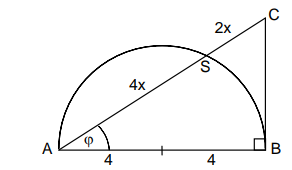
\includegraphics[scale=1]{trigo-thalesähnlichkeit.png}
\end{figure}


%---------------------------------------------------------
\question[3] % GZP 14 A9
Es gilt: \[\sin{(\alpha)}=\frac{4}{5}.\]
Berechne \begin{parts}
	\part $\cos{(\alpha)}$ \part $\tan{(\alpha)}$
\end{parts}
ohne den Winkel $\alpha$ explizit zu berechnen.


%---------------------------------------------------------
\question[4] % GZP 14 A15
\begin{minipage}{0.575\linewidth}
	Ein Aussichtsturm steht $30$m vom diesseitigen Kanalufer entfernt. Von der Aussichtsplattform $S$ aus erscheint das diesseitige Kanalufer unter einem Winkel von $\alpha=24.5^\circ$ und das jenseitige unter dem Winkel $\beta=64^\circ.$\vspace{5pt}
	\begin{parts}
		\part Wie hoch ist der Aussichtsturm?
		\part Wie breit ist der Kanal?
	\end{parts}
\end{minipage}
\hfill
\begin{minipage}{0.4\linewidth}
	\centering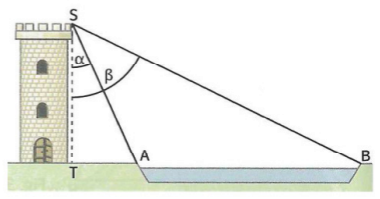
\includegraphics[scale=0.5]{trigo-aussichtsturm.png}
\end{minipage}


%---------------------------------------------------------
\question[4] % GZP 14 A17
Im rechtwinkligen Dreieck $ABC$ mit Hypotenuse $c$ sind die Seite $a=6$ und die Seitenhalbierende $s_a=13$ gegeben. Berechne die Höhe $h_c$.


%---------------------------------------------------------
\question[6] % GZP 15 A7
Kreuze an, ob die folgenden Aussagen oder Gleichungen richtig oder falsch sind.\\
\begingroup
\renewcommand{\arraystretch}{1.5}
\begin{table}[H]
	\centering
	\begin{tabular}{l|c|c}
		& richtig & falsch\\\hline
		$\sin{\alpha}=\sin{180^\circ-\alpha}$ & & \\
		$\cos{180^\circ-\beta}=\cos{180^\circ+\beta}$ & & \\
		$\tan{\alpha}>0$ für $90^\circ<\alpha<180^\circ$ & & \\
		$\cos{\alpha}=\sin{\alpha}$ für $\alpha=\frac{\pi}{6}$ & & \\
		$\sin{360^\circ-\beta}=\sin{180^\circ-\beta}$ & & \\
		In einem Dreieck mit $\gamma=90^\circ$ gilt: $\sin{\alpha}=\cos{90^\circ-\alpha}$ & & \\
	\end{tabular}
\end{table}
\endgroup

%---------------------------------------------------------
\question[3] % GZP 15 A16
In einem rechtwinkligen Dreieck $ABC$ mit Hypotenuse $c$ sind die Seite $a=7$ und die Seitenhalbierende $s_a=4.5$ gegeben. Berechne die Länge der Winkelhalbierenden $w_\beta$.


%---------------------------------------------------------
\question[4] % GZP 16 A12
Berechne \[\oldcos^2(\alpha)\*\tan{\alpha}-\oldsin^2(\alpha)\*\frac{1}{\tan{\alpha}}\]


%---------------------------------------------------------
\question[4] %GZP 18 A20
Im Rechteck $ABCD$ beträgt $\overline{AD}=10$cm, $\alpha=30^\circ$ und $\beta=70^\circ$. Berechne die Strecke $\overline{CE}$.
\begin{figure}[H]
	\centering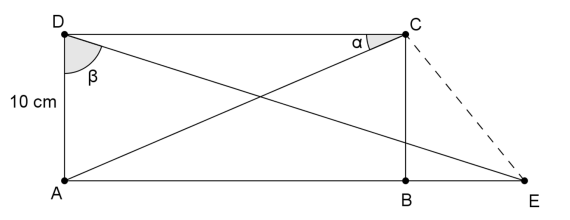
\includegraphics[scale=0.5]{trigo-rechteckstrecke.png}
\end{figure}


%---------------------------------------------------------
\question[3] % Barth Band 2 Kap. 5.7 A1d
Berechne die fehlenden Seitenlängen und Winkel im Dreieck $ABC$, wenn gilt: \[a=6,\quad b=5\quad\text{und}\quad \alpha=40^\circ.\]


%---------------------------------------------------------
\question[3] %Rhyn S9 A58
Von einem Parallelogramm $ABCD$ sind die Seiten $a=83$ und $b=109$ sowie die Diagonale $f=\overline{BD}=42$ gegeben. Berechne alle $4$ Innenwinkel dieses Parallelogramms?


%---------------------------------------------------------
\question[4] % Rhyn S6 A41
Ein Satellit befindet sich $100$km über dem Atlantik.\\
\textit{Tipp: } Der Erdradius beträgt $6370$km.
\begin{parts}
	\part Unter welchem Winkel ist der Rand der Erdkugel sichtbar?
	\part In welcher Entfernung ist der Rand der Erdkugel sichtbar?
\end{parts}

%---------------------------------------------------------
\question[3] % NW1 S188 A4
Welche der untenstehenden Winkel haben den gleichen Sinuswert?
\[\frac{\pi}{2},\qquad150^\circ, \qquad\frac{3\pi}{4}, \qquad90^\circ, \qquad\frac{\pi}{6}, \qquad45^\circ\]
Begründe mit Hilfe des Einheitskreises und ohne Verwendung des Taschenrechners.
\begin{figure}[H]
	\begin{tikzpicture}[cross/.style={draw, cross out, minimum size=2*(#1-1pt), inner sep=0pt, outer sep=0pt}, x=10mm, y=10mm,
		>=latex,   %Voreinstellung für Pfeilspitzen
		font= \footnotesize, scale=3]
		%Raster zeichnen
		% \draw [color=gray!50]  [step=7.5mm] (-1.3,-5.3) grid (14.8,5.8);
		% Achsen zeichnen
		\draw[->,thick] (-1.1,0) -- (1.2,0) node[right, below] {\normalsize $x$};
		\draw[->,thick] (0,-1.1) -- (0,1.2) node[above, left] {\normalsize $y$};
		% Achsen beschriften
		\foreach \x in {-1,1} \draw (\x,-.1) -- (\x,.1) node[below=4pt] {$\x$};
		\foreach \y in {-1,1} \draw (-.1,\y) -- (.1,\y) node[left=4pt] {$\y$};
		% Besserer Ursprung
		\draw[color=black] (0pt,-7pt) node[right] {$0$};
		%Funktionen zeichnen:
		\clip(-1.1,-1.1) rectangle (1.1,1.1); %Bildbereich
		\draw circle [radius=1];
	\end{tikzpicture}
\end{figure}


%---------------------------------------------------------
\question[4] % NW1 S188 A8
Welche der untenstehenden Winkel haben den gleichen Cosinuswert?
\[\frac{\pi}{2},\quad-270^\circ, \quad-120^\circ, \quad-90^\circ, \quad\frac{5\pi}{4}, \quad120^\circ, \quad135^\circ,\quad\frac{2\pi}{3}\]
Begründe mit Hilfe des Einheitskreises und ohne Verwendung des Taschenrechners.
\begin{figure}[H]
	\begin{tikzpicture}[cross/.style={draw, cross out, minimum size=2*(#1-1pt), inner sep=0pt, outer sep=0pt}, x=10mm, y=10mm,
		>=latex,   %Voreinstellung für Pfeilspitzen
		font= \footnotesize, scale=2.8]
		%Raster zeichnen
		%\draw [color=gray!50]  [step=2mm] (-1,-1) grid (1,1);
		% Achsen zeichnen
		\draw[->,thick] (-1.1,0) -- (1.3,0) node[right, below] {\normalsize $x$};
		\draw[->,thick] (0,-1.1) -- (0,1.3) node[above, left] {\normalsize $y$};
		% Achsen beschriften
		\foreach \x in {-1,1} \draw (\x,-.03) -- (\x,.03);
		\foreach \y in {-1,1} \draw (-.03,\y) -- (.03,\y);
		\draw[color=black] (1.05,-.1) node {$1$};
		\draw[color=black] (-.05,1.1) node {$1$};
		\draw[color=black] (-1.1,-.1) node {$-1$};
		\draw[color=black] (-.1,-1.1) node {$-1$};
		% Besserer Ursprung
		\draw[color=black] (0pt,-3pt) node[right] {$0$};
		% Funktionen zeichnen:
		\clip(-1.1,-1.1) rectangle (1.1,1.1); %Bildbereich
		\draw circle [radius=1];
	\end{tikzpicture}
\end{figure}


%---------------------------------------------------------
\question[4]
\begin{minipage}{0.6\linewidth}
	Du siehst von zwei verschiedenen Punkten, $A$ und $B$, die Spitze des Säntis. Beide Punkte befinden sich $400$m über Meer. Die Distanz zwischen $A$ und $B$ beträgt exakt $8.1$km. Beim Punkt $A$ siehst du die Spitze unter einem Winkel $\alpha=6^\circ$ und bei $B$ gilt $\beta=10^\circ$.\vspace{5pt}
	\begin{parts}
		\part Zeige rechnerisch, dass der Säntis ca. $2500$m hoch ist.
		\part Wie nahe bist du dem Säntis vom Punkt $B$?
	\end{parts}
\end{minipage}
\hfill
\begin{minipage}{0.35\linewidth}
	\centering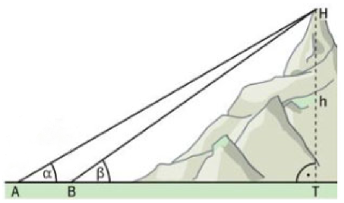
\includegraphics[scale=0.6]{trigo-aussichtspunkt.png}
\end{minipage}


%---------------------------------------------------------
\question[3]
Entscheide, ob die Aussagen in der Tabelle unten wahr oder falsch sind. Die Antworten müssen nicht begründet werden.\newline
\begin{small}
	Bewertung: Für $0-2$ richtige Antworten gibt es keine Punkte, $3$ richtige Antworten geben $1.5$ Punkte und falls alle Antworten richtig sind $3$ Punkte.
\end{small}
\begingroup
\renewcommand{\arraystretch}{1.5}
\begin{table}[H]
	\centering
	\begin{tabular}{|l|c|c|}\hline
		& wahr & falsch\\\hline
		$\sin{\alpha}=\sin{\pi-\alpha}$ & & \\\hline
		$\cos{\pi-\beta}=\cos{\pi+\beta}$ & & \\\hline
		$\tan{\alpha}>0$ für $90^\circ<\alpha<180^\circ$ & & \\\hline
		In einem Dreieck mit $\gamma=90^\circ$ gilt: $\sin{\alpha}=\cos{90^\circ-\alpha}$ & & \\\hline
		$\displaystyle\sin{90^\circ-\alpha}=\sin{90^\circ+\alpha}$ &  & \\\hline
		$\displaystyle\cos{\alpha}=-\cos{-\alpha}$ &  & \\\hline
		$\displaystyle\oldsin^2(\alpha)+\oldcos^2(\alpha)=\oldtan^2(\alpha)$ &  & \\\hline
		$\displaystyle\tan{270^\circ}$ ist nicht definiert. &  & \\\hline
	\end{tabular}
\end{table}
\endgroup




\end{questions}
\end{document}